\documentclass[]{../metanetpaper}

%!TEX TS-program = xelatex
\RequireXeTeX %Force XeTeX check


\title{Languages in the European Information Society}
\date{\today}
\author{Dr. John Doe (DFKI), Prof. Dr. Felix Sasaki (DFKI),\\
        Pepe Pérez (Academia de \LaTeX), Tan Ah Kao (USEV)}


\begin{document}

	\maketitle

	\section*{Preface}
	This white paper is part of a series that promotes knowledge about
language technology and its potential. It addresses educators, jour-
nalists, politicians, language communities and others.
The availability and use of language technology in Europe varies
between languages. Consequently, the actions that are required to
further support research and development of language technolo-
gies also differ for each language. The required actions depend on
many factors, such as the complexity of a given language and the
size of its community.
META-NET, a Network of Excellence funded by the European
Commission, has conducted an analysis of current language re-
sources and technologies. This analysis focused on the 23 official
European languages as well as other important national and re-
gional languages in Europe. The results of this analysis suggest that
there are many significant research gaps for each language. A more
detailed expert analysis and assessment of the current situation
will help maximise the impact of additional research and minimize
any risks.
META-NET consists of 47 research centres from 31 countries that
are working with stakeholders from commercial businesses, gov-
ernment agencies, industry, research organisations, software com-
panies, technology providers and European universities. Together,
they are creating a common technology vision while developing a
strategic research agenda that shows how language technology
applications can address any research gaps by 2020.

\clearpage

	\tableofcontents

	% 1.
	\clearpage
	\section{Executive Summary --- Zusammenfassung}
	

			Many European languages run the risk of becoming victims of the
digital age because they are underrepresented and under-resourced
online. Huge regional market opportunities remain untapped today
because of language barriers. If we do not take action now, many
European citizens will become socially and economically disadvan-
taged because they speak their native language.
Innovative language technology is an intermediary that will enable
European citizens to participate in an egalitarian, inclusive and
economically successful knowledge and information society. Multi-
lingual language technology will be a gateway for instantaneous,
cheap and effortless communication and interaction across lan-
guage boundaries.
Today, language services are primarily offered by commercial pro-
viders from the US. Google Translate, a free service, is just one
example. The recent success of Watson, an IBM computer system
that won an episode of the Jeopardy game show against human
candidates, illustrates the immense potential of language technolo-
gy. As Europeans, we have to ask ourselves several urgent ques-
tions:
\\
\begin {itemize}
\item Should our communications and knowledge infrastructure be
dependent upon monopolistic companies?
\item Can we truly rely on language-related services that can be im-
mediately switched off by others?
\item Are third parties from other continents willing to address our
translation problems and other issues that relate to European
multilingualism?
\item Can our European cultural background help shape the
knowledge society by offering better, more secure, more precise,
more innovative and more robust high-quality technology?
\end {itemize}
This whitepaper for the German language demonstrates that a lan-
guage technology research and development community exists in
Germany, Austria and Switzerland. However, many large compa-
nies have stopped their activities in language technology research
and development, which is nowadays almost exclusively performed
by small and medium enterprises that can hardly compete on the
global market. While Germany used to be a European hub in this
area in the past, we now have to ask ourselves if we want to actively
compete in the global market for research and development in this
future technology or not.
Although a number of technologies and resources for Standard
German exist, there are fewer technologies and resources for the
German language than for the English language. The existing tech-
nologies and resources are also poorer in quality.
According to the assessment detailed in this report, immediate
action must occur before any breakthroughs for the German lan-
guage can be achieved.\\
	\section{Risk for Our Languages and a Challenge for Language Technology}
	We are witnesses to a digital revolution that is dramatically impact-
ing communication and society. 
\margin{We are currently witnessing a
digital revolution that is compara-
ble to Gutenberg’s invention of the
printing press.}
\\Recent developments in digital
information and communication technology are sometimes com-
pared to Gutenberg’s invention of the printing press. What can this
analogy tell us about the future of the European information socie-
ty and our languages in particular?\\
After Gutenberg’s invention, real breakthroughs in communication
and knowledge exchange were accomplished by efforts such as
Luther’s translation of the Bible into vernacular language. In sub-
sequent centuries, cultural techniques have been developed to bet-
ter handle language processing and knowledge exchange:
\begin{itemize}
\item the orthographic and grammatical standardisation of major
   languages enabled the rapid dissemination of new scientific and
  intellectual ideas;
\item the development of official languages made it possible for citi-
   zens to communicate within certain (often political) boundaries;
\item the teaching and translation of languages enabled exchanges
   across languages;
\item the creation of editorial and bibliographic guidelines assured
   the quality and availability of printed material;
\item the creation of different media like newspapers, radio, televi-
   sion, books, and other formats satisfied different communica-
  tion needs.
In the past twenty years, information technology has helped to
automate and facilitate many of the processes:
\item desktop publishing software has replaced typewriting and type-
   setting;
\item Microsoft PowerPoint has replaced overhead projector trans-
   parencies;
\item e-mail send and receive documents faster than a fax machine;
\item Skype offers cheap Internet phone calls and hosts virtual meet-
   ings;
\item audio and video encoding formats make it easy to exchange
   multimedia content;
\item search engines provide keyword-based access to web pages;
\item online services like Google Translate produce quick, approxi-
   mate translations;
\item social media platforms such as Facebook, Twitter, and Google+
   facilitate communication, collaboration, and information shar-
  ing.
\end{itemize}
Although such tools and applications are helpful, they are not yet
capable of supporting a sustainable, multilingual European society
for all where information and goods can flow freely.
\subsection{Language Borders Hinder the European
Information Society}
We cannot predict exactly what the future information society will
look like. But there is a strong likelihood that the revolution in
6
communication technology is bringing people speaking different
languages together in new ways. This is putting pressure on indi-
viduals to learn new languages and especially on developers to
create new technology applications to ensure mutual understand-
ing and access to shareable knowledge.\\
\margin{A global economy and information
space confronts us with more lan-
guages, speakers and content.}
In a global economic and
information space, more languages, speakers and content interact
more quickly with new types of media. The current popularity of
social media (Wikipedia, Facebook, Twitter, YouTube, and, recent-
ly, Google+) is only the tip of the iceberg. Today, we can transmit gigabytes of text around the world in a few
seconds before we recognize that it is in a language we do not un-
derstand. According to a recent report from the European Commission, 57\% of Internet users in Europe purchase goods and services
in languages that are not their native language. (English is the most
common foreign language followed by French, German and Span-
ish.) 55\% of users read content in a foreign language while only
35\% use another language to write e-mails or post comments on
the Web.i A few years ago, English might have been the lingua fran-
ca of the Web — the vast majority of content on the Web was in Eng-
lish — but the situation has now drastically changed. The amount of
online content in other European (as well as Asian and Middle
Eastern) languages has exploded.
Surprisingly, this ubiquitous digital divide due to language borders
has not gained much public attention; yet, it raises a very pressing
question: Which European languages will thrive in the networked
information and knowledge society, and which are doomed to dis-
appear?

\subsection{Our Languages at Risk}
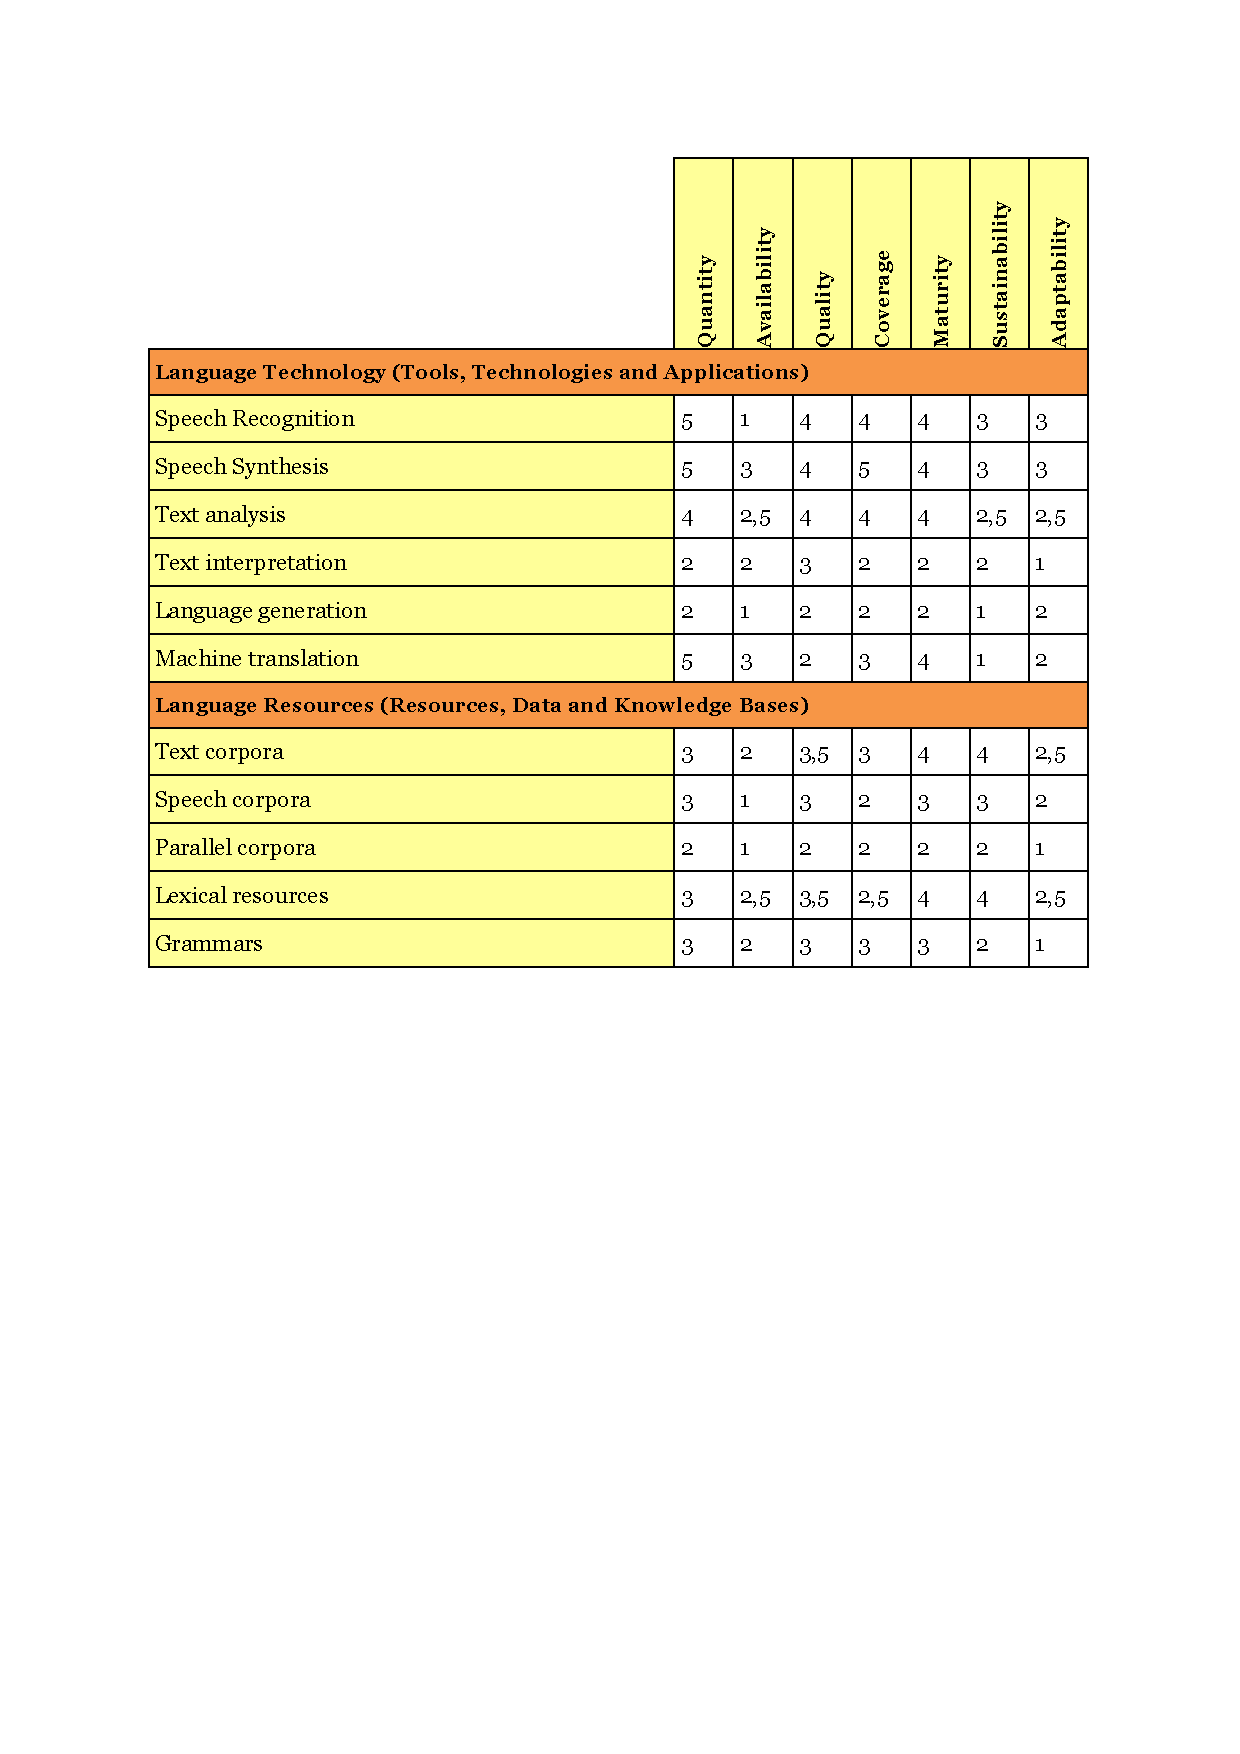
\includegraphics[scale=0.75]{../media/metanet-paper2.pdf} 
While the printing press helped step up the exchange of infor-
mation in Europe, it also led to the extinction of many European
languages. Regional and minority languages were rarely printed
and languages such as Cornish and Dalmatian were limited to oral
forms of transmission, which in turn restricted their scope of use.
Will the Internet have the same impact on our languages?
Europe’s approximately 60 languages are one of its richest and
most important cultural assets, and a vital part of its unique social
model.\footnote{European Commission, Multilingualism: an asset for Europe and a shared commitment, Brussels,
2008 (http://ec.europa.eu/education/languages/pdf/com/2008\_0566\_en.pdf).}
\margin{The wide variety of languages in
Europe is one of its richest and most
important cultural assets.} While languages such as English and Spanish are likely to
survive in the emerging digital marketplace, many European lan-
guages could become irrelevant in a networked society. This would
weaken Europe’s global standing, and run counter to the strategic
goal of ensuring equal participation for every European citizen
regardless of language. According to a UNESCO report on multilin-
gualism, languages are an essential medium for the enjoyment of
fundamental rights, such as political expression, education and
participation in society.\footnote{UNESCO Director-General, Intersectoral mid-term strategy on languages and multilingualism, Paris, 2007 (http://unesdoc.unesco.org/images/0015/001503/150335e.pdf).}
\subsection{Language Technology is a Key Enabling Technology}
In the past, investment efforts in language preservation focused on
language education and translation. According to one estimate, the
European market for translation, interpretation, software localisa-
tion and website globalisation was €8.4 billion in 2008 and is ex-
pected to grow by 10\% per annum.iv Yet this figure covers just a
small proportion of current and future needs in communicating
between languages. \margin {Language technology helps people
collaborate, conduct business, share
knowledge and participate in social
and political debates across differ} The most compelling solution for ensuring the
breadth and depth of language usage in Europe tomorrow is to use appropriate technology, just as we use technology to solve our
transport, energy and disability needs among others.
Digital language technology (targeting all forms of written text and
spoken discourse) helps people collaborate, conduct business,
share knowledge and participate in social and political debate re-
gardless of language barriers and computer skills. It often operates
invisibly inside complex software systems to help us:
\begin{itemize}
\item find information with an Internet search engine;
\item check spelling and grammar in a word processor;
\item view product recommendations in an online shop;
\item hear the verbal instructions of a car navigation system;
\item translate web pages via an online service.
\end{itemize}
Language technology consists of a number of core applications that
enable processes within a larger application framework. The pur-
pose of the META-NET language white papers is to focus on how
ready these core technologies are for each European language.
\margin {Europe needs robust and affordable
language technology for all European languages.}
To maintain our position in the frontline of global innovation, Eu-
rope will need language technology adapted to all European lan-
guages that is robust, affordable and tightly integrated within key
software environments. Without language technology, we will not
be able to achieve a really effective interactive, multimedia and
multilingual user experience in the near future.
\subsection{Opportunities for Language Technology}
In the world of print, the technology breakthrough was the rapid
duplication of an image of a text (a page) using a suitably powered
printing press. Human beings had to do the hard work of looking
up, reading, translating, and summarizing knowledge. We had to
wait until Edison to record spoken language – and again his tech-
nology simply made analogue copies.
Digital language technology can now automate the very processes
of translation, content production, and knowledge management for
all European languages. It can also empower intuitive lan-
guage/speech-based interfaces for household electronics, machin-
ery, vehicles, computers and robots. Real-world commercial and
industrial applications are still in the early stages of development,
yet R\&D achievements are creating a genuine window of oppor-
tunity. For example, machine translation is already reasonably
accurate in specific domains, and experimental applications pro-
vide multilingual information and knowledge management as well
as content production in many European languages.
As with most technologies, the first language applications such as
voice-based user interfaces and dialogue systems were developed
for highly specialised domains, and often exhibit limited perfor-
mance. But there are huge market opportunities in the education
and entertainment industries for integrating language technologies
into games, cultural heritage sites, edutainment packages, libraries,
simulation environments and training programmes. Mobile infor-
mation services, computer-assisted language learning software,
eLearning environments, self-assessment tools and plagiarism
detection software are just some of the application areas where
language technology can play an important role.
\margin {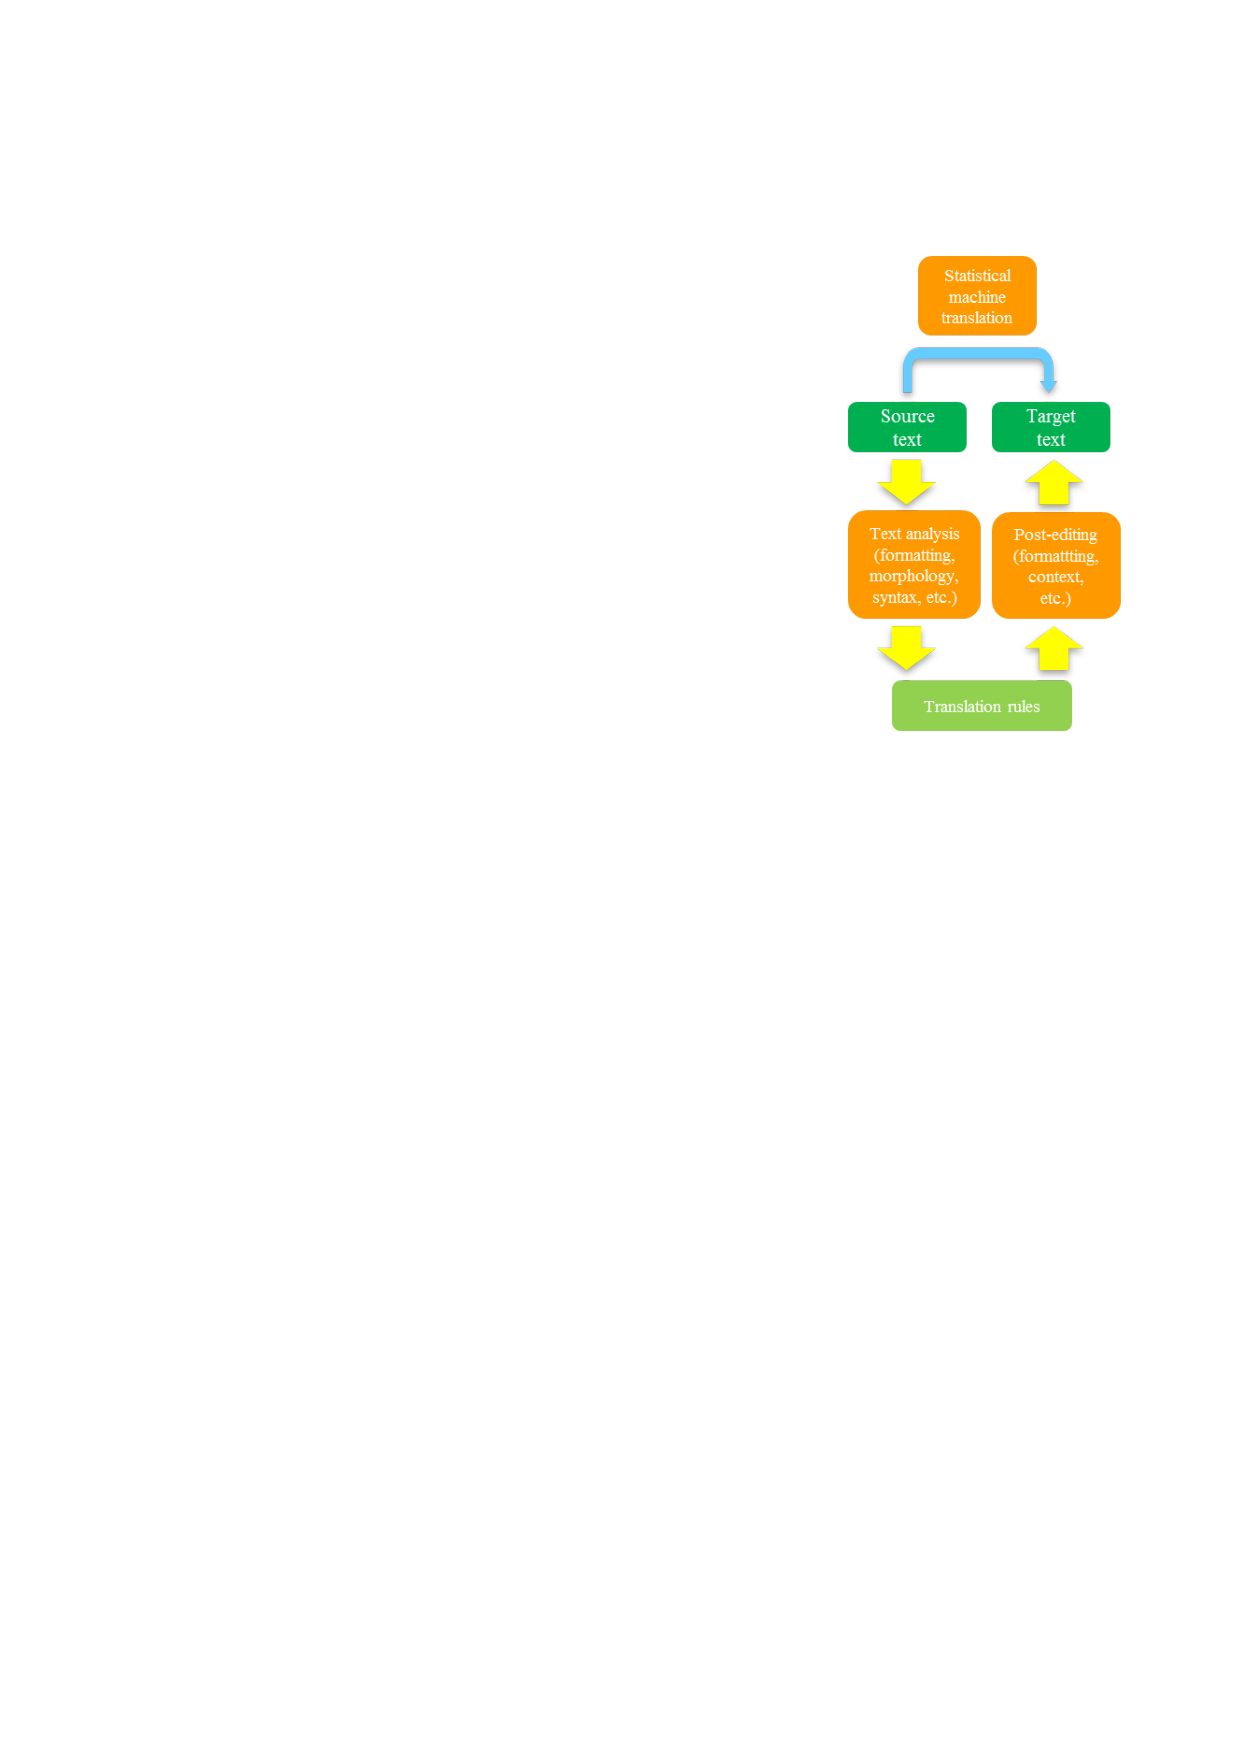
\includegraphics[scale=1]{../media/metanet-paper.pdf} }
The popularity of social media applications like Twitter and Facebook suggest a fur-
ther need for sophisticated language technologies that can monitor
posts, summarise discussions, suggest opinion trends, detect emo-
tional responses, identify copyright infringements or track misuse.


\end{document}
